% !TEX root = ../thesis.tex
%
\chapter{Concepts}
\label{sec:concepts}

\cleanchapterquote{Q: What's the difference between machine learning and statistics?\\A: ConvNets}{Bored Yann LeCun}{via Twitter}

\section{Task definitions}
\label{sec:concepts:tasks}
Although the posed task for this thesis is pretty clear from its formulation, we want to quickly distinguish the similar but different image understanding tasks that are solved using these techniques.

The simplest task that was tackled is \textbf{image classification}. In image classification the input are images $I$ containing a single object that fills most of the image. Hence the task is to find the class label $c$ for the singular object $o$ which therefore labels the whole image: $f(I) = c_o$. Since 2015 \glspl{cnn} can surpass the performance of humans doing classification \citep{he_delving_2015}.

Next \textbf{object localization} was addressed. Localization means that we still have only one relevant object per image $I$ but here the object fills only a part of the image. Instead of only predicting the class $c$ for this object $o$ the localizer also has to predict translation $t$ and scaling $s$ for the object: $f(I) = (c, t, s)_o$.

Harder to solve but also way more applicable is \textbf{object detection}. Now we take complicated images $I$, containing a variable number of possibly overlapping objects $O = \{o_1,o_2,\dotsc,o_n\}$, each of varying class $c$. The detector has to identify and localize all objects inside the image: $f(I) = \{(c, t, s)_1, (c, t, s)_2,\dotsc,(c, t, s)_n\}$.

Lastly we have \textbf{image segmentation}. Here we aim to not only identify multiple different objects $o$ in an image $I$ but also to find their boundaries on the pixel level: f(I) =$ \{ c_i\ \forall i \in I\}$. As such each pixel of a found object in the image is labeled with its class label resulting in multiple binary masks each masking out one individual object.

\section{Neural Networks}
\label{sec:concepts:nn}
Neural networks are a specific method to approximate a function $f(x) = y$, which yields some desired output from input data. For example this could be the task to return the name of the breed given images of dogs as input. They are called networks because they are a composite of chained functions, each computing one step of the overall function. Data flows from the top, the first computation, to the end getting further processed: $f(x) = f_n(f_{n-1}(\dots f_1(x))) = y$. When the network is connected on a acyclic graph, meaning the flowing data does not go through any loops, it is called a \textbf{feedforward network}.\\
\TODO{glue}

Working on raw pixel values of images, it will, in the most cases, not be possible to find a linear decision function which separates inputs according to the task \citep{lecun_deep_2015}. To discriminate such representation we need a non-linear decision boundary and thus a neural network should be a composite of linear and non-linear operations, so that it, at least in theory, can approximate the non-linear representation.

\subsection{Gradient descent}
\label{sub:concepts:nn:gd}
\TODO{write section}

\subsection{Backpropagation}
\label{sub:concepts:nn:backprob}
\citet{rumelhart_learning_1988}
computing the gradient then used to apply a gradient descent method
\TODO{write section}

\subsection{Convolution} % (fold)
\label{sub:conepts:nn:conv}
Convolution is a special kind of linear operation, that is successfully applied in deep neural networks, which we then call a \acrfull{cnn}. For two one-dimensional continuous signals expressed by the functions $f$ and $g$ their convolution is described as follows:
\begin{equation}
    (f * g)(t) = \int_{-\infty}^\infty f(\tau)g(t - \tau)d\tau
\end{equation}
Here the function $g$ is translated through the functions domain and we integrate over the piecewise multiplication of the shifting $g$ and the stationary $f$.
Because we work on digital discretized data (\textit{e.g. images}) we need the discretized convolution which in $1d$ looks like this:
\begin{equation}
    (I * K)(t)  = \sum_{\tau = - \infty}^\infty I(\tau)K(t - \tau)
\end{equation}
Again we see how $K$ slides over the domain of $I$ and $K$, and is multiplicated at each step with $I$.\\
We want to use convolutions to examine images. While images could be flatted into a $1d$ representation that would drop $2d$ visual information. As such we want to use convolutions on $2d$ signals:
\begin{equation}
    (I * K)(x,y)  = \sum_i\sum_j I(x,y)K(x-i,y-j)
\end{equation}
$I$ is the input, an image, and $K$ is called the \textbf{kernel}. The kernel is shifted over both axes of the image and at each position we compute the multiplication between the kernel and the respective part of the image. For example $K$ could be of size $3\times 3$ pixels and for an arbitrarily sized image $I$, the convolution $I * K$ would return all results of the multiplication between $K$ and each $3 \times 3$ pixel sized window of the image, around each pixel $i(x,y)$ inside $I$. The part of the input image that the kernel is connected to at one computation is called its \textbf{receptive field}. The result can be seen as  a map, same-sized to the input, describing how much the input responded to the kernel at each point, thus it often is called \textbf{response map}.

The first advantage in the use of kernels is that they can remain very small (like $3\times 3$ pixels or $7\times 7$ pixels) but return outputs for the way bigger input and therefore need few parameters to operate. Secondly convolutions are equivariant to translations which means that if we translate the input somehow, the response, at the shifted position in the response map, is still the same as before. This is really important because then the convolutions respond to signals independent of their position in the input image.Lastly convolutions can be described with a value restricted matrix multiplication, in the form of a Toeplitz matrix, and therefore the discretized convolution is a linear operation. Using many optimizations from linear algebra convolutions can be computed immensely fast.\\
Inside \glspl{cnn} we use convolutions to map, how much a specific small structure is present at each position inside a image. An example of this is shown in \figreft{fig:sigmoid_relu}.

\subsection{Activation Functions} % (fold)
\label{sub:conepts:nn:activations}
\begin{figure}
    \centering
    \begin{tabulary}{\linewidth}{CCCC}
        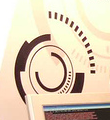
\includegraphics[height=3cm]{figures/activation_data} &
        \vspace{-1.8cm}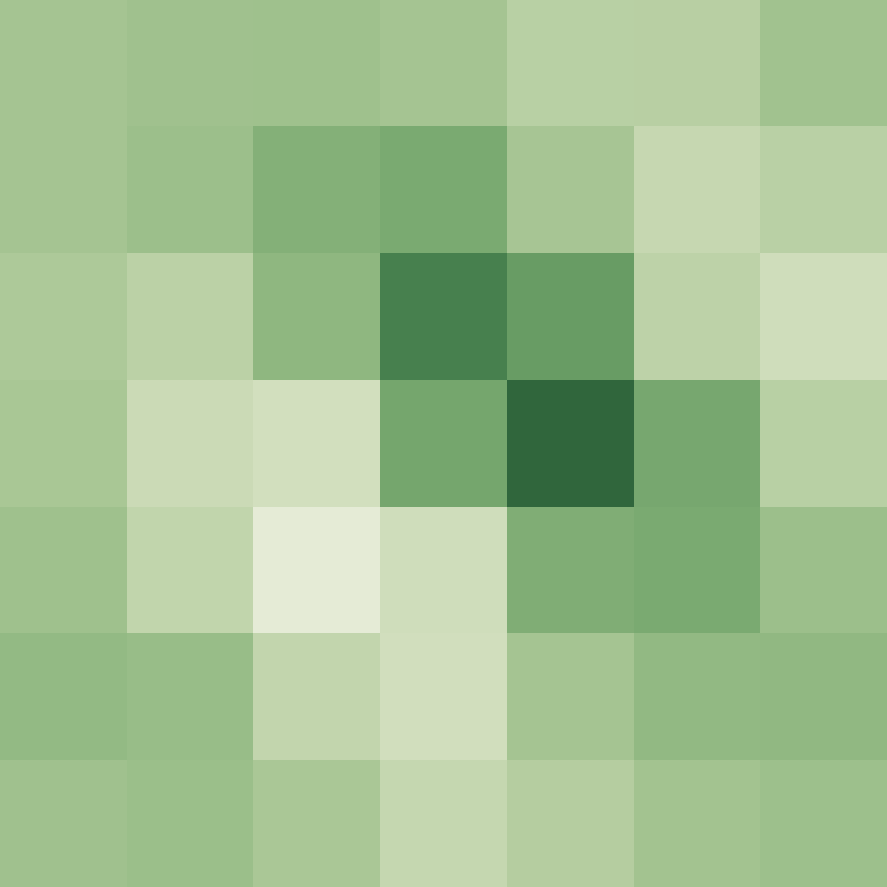
\includegraphics[height=1cm]{figures/activation_filter} &
        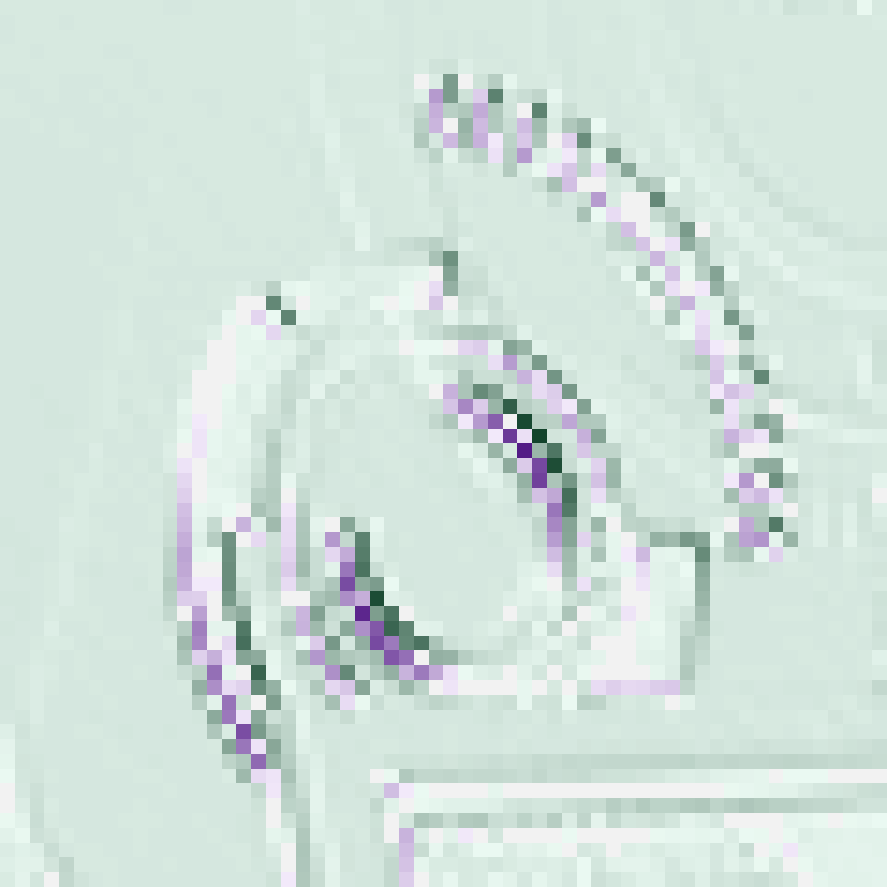
\includegraphics[height=3cm]{figures/activation_response} &
        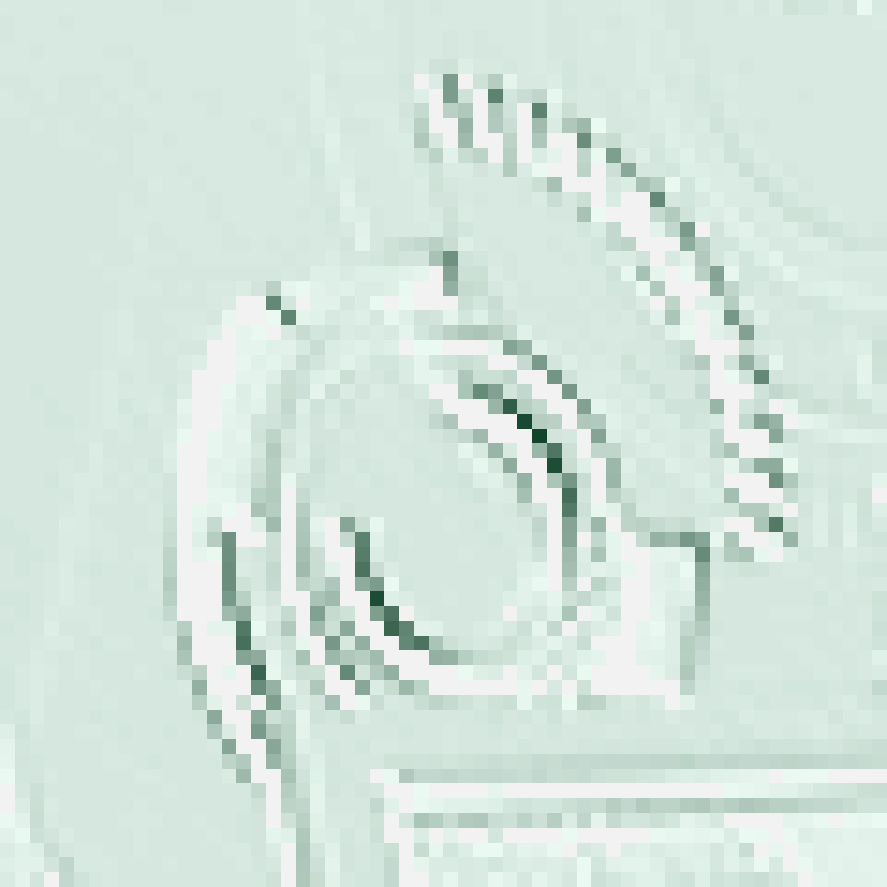
\includegraphics[height=3cm]{figures/activation_relu} \\
        image data & filter & filter response & \gls{relu} \\
    \end{tabulary}
    \caption{The effect of a convolution and a following \gls{relu} visualized. The green activations are positive and the purple ones are negative.}
\end{figure}
\begin{figure}
    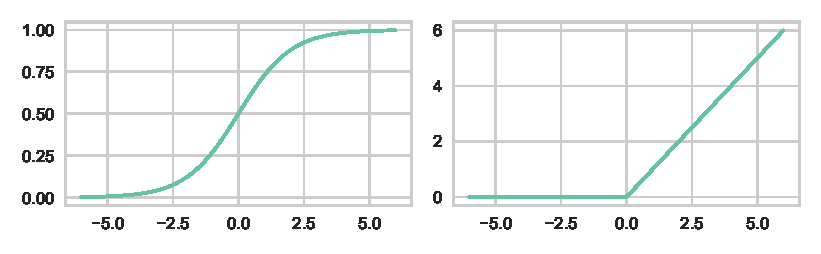
\includegraphics{figures/sigmoid_relu}
    \caption{Activation functions: sigmoid on the left and rectifier from a \gls{relu} on the right.}
    \label{fig:sigmoid_relu}
\end{figure}
\gls{conv} layers return the response of their inputs to their filters. Next the response level is used to calculate how much the node in the network fires for this position. Conceptually this draws from the activation process inside neurons in the brain, which also receive inputs from their dendrites and fire along their axon. Inside an artificial neural network this mapping is done by an activation function $f(x)$. In the most simple cases this can be the identity $f(x) = x$ or the unit step function $f(x) = (\sign x + 1) / 2$. With the identity we just use the response values as firing rates not introducing any more complexity and the sign reduces the levels of response to a binary firing switch.

Formerly common to use as an activation function was the sigmoid. The sigmoid $\sigma(x) = 1/(1+e^{-x})$ \fref{fig:sigmoid_relu} takes an unbounded input range and squashes it into the range $[0, 1]$. Today sigmoids are mostly avoided as they hold multiple drawbacks. First as the function values saturate in both directions its gradient can approximate zero, which with backpropagation can lead to zeroed gradients or exploding gradients while training. Secondly the gradient computation is slow due to its non-linear form.

One popular function to hold those properties is the rectifier \fref{fig:sigmoid_relu}
\begin{equation}
    \rho(x) = max(0, x)
\end{equation}
employed in \glspl{relu}. While being piecewise linear, and thus still computationally efficient, the rectifier is a non-linear function and can fold the decision space into a non-linear form. Because it does not saturate like the sigmoid it avoids the problems of zeroed or exploding gradients.

\subsection{Pooling}
\label{sub:concepts:nn:pooling}
A typical building block for \glspl{cnn} is the triple of a \gls{conv} layer, followed by a non-linear activation function, followed by a pooling layer. The pooling layer takes its input from the previous layer and compresses it spatially into into a smaller form. Different functions can be applied to the data neighborhood from the input. Average pooling \citep{lecun_handwritten_1990} or max pooling \citep{zhou_computation_1988} are two of the most prominent ones. With average pooling we return the average of the values from the neighborhood and with max pooling we return the maximum value from the neighborhood.

It is important to note that average pooling is a linear function while max pooling is not. Pooling can be used to introduce more non-linearity and that is one reason while max pooling is more popular to use. Also as downsampling of the deep filters can be done with strided convolutions alone, pooling is not necessary needed for this and more and more network architectures drop the pooling layers entirely \citep{springenberg_striving_2014}.

\subsection{Batch Normalization} % (fold)
\label{sub:conepts:nn:batchnorm}
Batch normalization \citep{ioffe_batch_2015} is a method to ease the computation of gradient descent in backpropagation and also to reduce problems of bad weight initialization. Inside training of a deep network emerges the problem of internal covariate shift. Each deeper layer of the network depends on the outputs from its previous layer. The first layer learns on top of the data input, but the second layer learns from the output of the first layers features, and the third layer depends on the second one and so on. In training all these features change through backpropagation and the distribution of all activations change and the deeper the layer is, the longer the chain of evolving distributions in front of it becomes.\\
If the features in training shift over time the gradient decent becomes harder as each layer has to follow this covariate shift of its successor. BatchNorm helps to avoid this difficulty by normalizing mini batches of inputs. The layer is added after a convolutional layer (or any other linear layer) and collects a batch of output samples $X = \{x_1, x_2, x_3, \dots, x_n\}$. Then it calculates the mean $\mu_X$ and the variance $\sigma_X^2$ for this mini batch. Normalizing all the values from that batch with
\begin{equation}
    \hat{x_i} = \frac{x_i - \mu_X}{\sqrt{\sigma_X^2 + \epsilon}}
\end{equation}
($\epsilon$ is added to avoid divisions by zero) yields the output $\{\hat{x_1},\dots,\hat{x_n}\}$.\\
To use the BatchNorm parameters while testing, we compute a moving average over the means and variances of the batches while training. The forward pass uses these averages to normalize the test inputs.

\section{Fully Convolutional Networks}
\label{sec:concepts:fcn}
Proposed by \citet{long_fully_2015}, \glspl{fcn} are a specific architecture of \glspl{cnn}. Fully convolutional states that the network consists only of convolutional layers. As these are translation invariant the networks can take arbitrarily sized inputs and produce an dependently sized coarse output.

The original authors use this architecture for image segmentation. They build their network from classic semantic object classifiers like VGG-16 \citep{simonyan_very_2014}. These take fixed sized images as inputs and produce a single label thereby classifying the whole image. Typically these networks produce high level features through a series of convolutional layers and classify them with a single or a series of \gls{fc} layers. To label an image pixel-wise with such an architecture we would have to forward the neighborhood of each pixel through the network which would introduce an \bigO{w * h} time complexity ($w$ and $h$ being the width and the height of the image).

\subsection{Transposed Convolution} % (fold)
\label{sub:conepts:fcn:deconv}

\begin{figure}[h]
    \centering
    \begin{tabular}{cc}
    \begin{tikzpicture}[font=\footnotesize\sffamily]
        \fill[black!20] (1,3) rectangle (2,3.5);
        \fill[black!20] (6,3) rectangle (7,3.5);

        \foreach \x/\y in {1/2, 2/1.5, 3/1, 4/0.5, 5/0}
            \fill[set2_1!50] (\x, \y) rectangle (\x + 2, \y + 0.5);

        \fill[black!20] (1,2) rectangle (2,2.5);
        \fill[black!20] (6,0) rectangle (7,0.5);

        \foreach \x/\y in {1/2, 2/1.5, 3/1, 4/0.5, 5/0}
        {
            \node[above right] at (\x + 0.0, \y) {1};
            \node[above right] at (\x + 0.5, \y) {2};
            \node[above right] at (\x + 1.0, \y) {3};
            \node[above right] at (\x + 1.5, \y) {4};
        }

        \draw[step=0.5cm,gray,very thin] (0,0) grid (0.5,2.5);
        \draw[step=0.5cm,gray,very thin] (0.99,2.99) grid (7,3.5);
        \draw[step=0.5cm,gray,very thin] (0.99,0) grid (7,2.5);
        \draw [->] (2.25,3.25) -- (2.25,2);
        \draw [->] (2.75,3.25) -- (2.75,2);
        \draw [->] (3.25,3.25) -- (3.25,2);
        \draw [->] (3.75,3.25) -- (3.75,2);
        \draw [->] (1.9,1.75) -- (0.5,1.75);
    \end{tikzpicture} &
    \begin{tikzpicture}[font=\footnotesize\sffamily]
        \fill[black!20] (0,5) rectangle (0.5,6);
        \fill[black!20] (0,0) rectangle (0.5,1);

        \foreach \y/\x in {4/1, 3/1.5, 2/2, 1/2.5, 0/3}
            \fill[set2_1!50] (\x, \y) rectangle (\x + 0.5, \y + 2);

        \fill[black!20] (1,5) rectangle (1.5,6);
        \fill[black!20] (3,0) rectangle (3.5,1);

        \foreach \y/\x in {4/1, 3/1.5, 2/2, 1/2.5, 0/3}
        {
            \node[above right] at (\x, \y + 1.5) {1};
            \node[above right] at (\x, \y + 1.0) {2};
            \node[above right] at (\x, \y + 0.5) {3};
            \node[above right] at (\x, \y) {4};
        }

        \draw[step=0.5cm,gray,very thin] (0.99,6.49) grid (3.5,7);
        \draw[step=0.5cm,gray,very thin] (0,0) grid (0.5,6);
        \draw[step=0.5cm,gray,very thin] (0.99,0) grid (3.5,6);
        \draw [->] (1.25,6.75) -- (1.25,5);
        \draw [->] (1.75,6.75) -- (1.75,5);
        \draw [->] (1,4.75) -- (0.5,4.75);
        \draw [->] (1,4.25) -- (0.5,4.25);
    \end{tikzpicture} \\[6pt]
    (a) Convolution & (b) Transposed Convolution
    \end{tabular}
    \caption{Convolution with stride 2 in 1D and transposed convolution with stride 2. Input signals are at the top, output is to the right and the gray boxes are padding. With the arrows we note how input points contribute to the output. The convolution applies a filter of size 4 to an signal of size 8 and with the padding produces an output of size 5. The transposed convolution in return takes a input of 5 and returns a signal of size 10. Figure is based on \citep{shi_is_2016}.}
    \label{fig:1d_strided_conv}
\end{figure}

Transposed convolution or sometimes mistakenly called deconvolution, first used by \citet{zeiler_deconvolutional_2010}, introduces a new operation for neural networks. Simply spoken a transposed convolution takes the receptive field and produces a larger window as output, thus operating some form of upsampling. \figreft{fig:1d_strided_conv} visualizes the differences between convolution and transposed convolution in $1d$.
\TODO{finish section}

\subsection{Conversion of \gls{fc} layers}
\label{sub:concepts:fcn:fc_conversion}
\gls{fc} layers can directly be converted into \gls{conv} layers, which makes \glspl{fcn} immensely efficient. To understand this process let us examine the VGG-16 network. After the 13 \gls{conv} layers and 5  corresponding max-pooling layers we get an output from \texttt{pool5} with $512\times7\times7$ pixels. Through pooling the original images ($224\times224$ pixels) got reduced to $7\times7$ pixels images over 512 channels. These go though 3 \gls{fc} layers. The first \gls{fc} layer returns 4096 values. We replace it with a \gls{conv} layer with kernel size 7 and 4096 channels thus also resulting in an $1\times1\times4096$ pixels output. The weights from the \gls{fc} layer can be reshaped into the size of the \gls{conv} layer. The other two \gls{fc} layers with 4096 and 1000 outputs, respectively can directly be put into convolutions with kernel size 1.

For the former images of $224\times224$ pixels nothing changed as the output of the first \gls{fc} layer is still 4096 values but if we now increase the data size to e.g. the double $448\times448$ pixels, the advantage becomes apparent. The \texttt{pool5} will return outputs of size $14\times14$ pixels and the new \gls{conv} layer will slide over the bigger images returning outputs of size $8\times8$ pixels. Lastly the other $1\times1$ pixel-sized convolutions do not change the size so that we get 64, spatially located, predictions over the 1000 classes instead of one. These are the same as if we would have slided a window over the original image with an $8\times8$ grid but because the computations on the GPU are shared for the convolutional kernels we heavily increased performance compared to the naïve solution.

\subsection{Upsampling through Convolutions}
\label{sub:concepts:fcn:upsampling}
A \gls{fcn} as in \citep{long_fully_2015} outputs a small sparse score map. For an input image of $200\times 200$ pixels, that could be something around $10\times 10$ values. Naturally we want an output map with the same size as the input. Firstly we can use feature maps from earlier layers with their own classifiers to reduce the stride of the resulting score map but the score map from deeper layers has still to be upsampled to the input size. Upsampling can be done directly within the network using convolutions. It is possible to use transposed convolutions to upsample the inputs and filter them at the same time but this often introduces artifacts \citep{odena_deconvolution_2016}. Alternatively refining e.g. bilinear kernels in training does not help much in performance \citep{shelhamer_fully_2016}. It seems successful to upsample the score maps with a normal interpolation followed by normal convolutions at the bigger size \citep{dong_image_2016}.

\section{Residual Networks}
\label{sec:concepts:resnet}
After the success of AlexNet \citep{krizhevsky_imagenet_2012} and with the possibilities of fast GPU computing, neural networks got deeper and bigger.
The VGG-16 by \citet{simonyan_very_2014} has 442.5 million trainable parameters for its 16 layers. The more parameters a network has the harder the training becomes.
For the last years multiple new network architectures have been developed that achieve higher accuracy needing less parameters and therefore shorter inference time \citep{canziani_analysis_2016}. One of those architectures are \glspl{resnet} by \citet{he_deep_2016} with which they won the COCO  \citet{lin_microsoft_2014} and the ImageNet \citet{russakovsky_imagenet_2015}  challenges in 2015.
A \gls{conv} layer in a standard feed forward network learns a mapping $\mathcal{H}(x)$ from its input $x$. When training the network we reach the point at which the accuracy saturates. At this point the layers which are still being trained should approximate an identity mapping of their inputs as the optimum has already been reached. In practice with deep networks, new layers, at some point in training, rapidly move away from the identity they should learn and degrade the training error after it already saturated. Thus making these networks deeper will worsen their results \citep{he_convolutional_2015}.
\begin{figure}
    \centering
    \begin{tabular}{p{6cm}p{6cm}}
    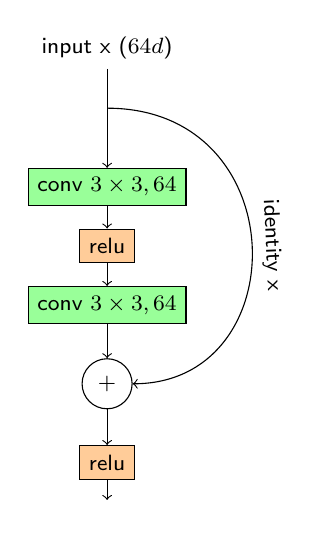
\begin{tikzpicture}[font=\footnotesize\sffamily]
        \path (0, 5) node[above](xinp) {input x ($64d$)}
              (0, 3.5) node[fill=green!40, draw](xc1) {\gls{conv} $3\times3, 64$}
              (0, 2.75) node[fill=orange!40, draw](xr1) {\gls{relu}}
              (0, 2) node[fill=green!40, draw](xc2) {\gls{conv} $3\times3, 64$}
              (0, 1) node[circle,draw](xplus) {+}
              (0, 0) node[fill=orange!40, draw](xend) {\gls{relu}}
              (0, -0.6) node(xout) {};
        \draw[->] (xinp) -- (xc1);
        \draw[->] (xc1) -- (xr1);
        \draw[->] (xr1) -- (xc2);
        \draw[->] (0, 4.5) .. controls +(right:2.4cm) and +(right:2.4cm) .. node[sloped, above] {identity x} (xplus);
        \draw[->] (xc2) -- (xplus);
        \draw[->] (xplus) -- (xend);
        \draw[->] (xend) -- (xout);
    \end{tikzpicture} &

    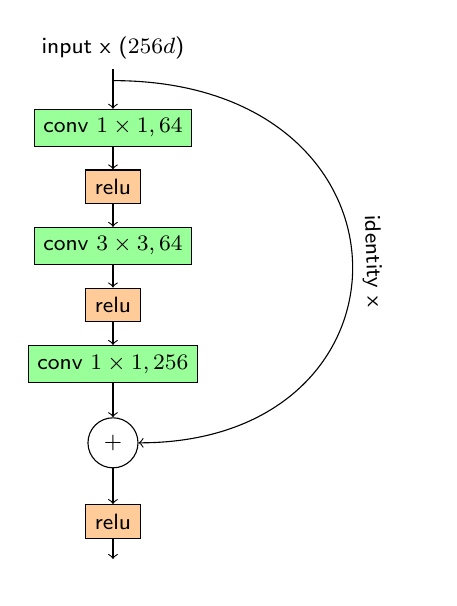
\begin{tikzpicture}[font=\footnotesize\sffamily]
        \path (0, 5.75) node[above](xinp) {input x ($256d$)}
              (0, 5) node[fill=green!40, draw](xc1) {\gls{conv} $1\times1, 64$}
              (0, 4.25) node[fill=orange!40, draw](xr1) {\gls{relu}}
              (0, 3.5) node[fill=green!40, draw](xc2) {\gls{conv} $3\times3, 64$}
              (0, 2.75) node[fill=orange!40, draw](xr2) {\gls{relu}}
              (0, 2) node[fill=green!40, draw](xc3) {\gls{conv} $1\times1, 256$}
              (0, 1) node[circle,draw](xplus) {+}
              (0, 0) node[fill=orange!40, draw](xend) {\gls{relu}}
              (0, -0.6) node(xout) {};
        \draw[->] (xinp) -- (xc1);
        \draw[->] (xc1) -- (xr1);
        \draw[->] (xr1) -- (xc2);
        \draw[->] (xc2) -- (xr2);
        \draw[->] (xr2) -- (xc3);
        \draw[->] (0, 5.6) .. controls +(right:4cm) and +(right:4cm) .. node[sloped, above] {identity x} (xplus);
        \draw[->] (xc3) -- (xplus);
        \draw[->] (xplus) -- (xend);
        \draw[->] (xend) -- (xout);
    \end{tikzpicture}
    \\[6pt]
    (a) A simple non-linear residual block. & (b) A bottleneck block as employed in the deeper \glspl{resnet}.
    \end{tabular}

    \caption{Two examples of residual blocks. The input of the block is fused into the ouptut of the last \gls{conv} layer and added element-wise channel-per-channel onto it. A \gls{relu} is trailing the sum again.}
    \label{fig:resblock}
\end{figure}


The main idea of \glspl{resnet} is pretty simple. They are built from many small identical blocks \fref{fig:resblock}. Instead of blocks that learn the mapping $\mathcal{H}(x)$ we introduce blocks that learn the \textit{residual} $\mathcal{F}(x) = \mathcal{H}(x) - x$ of this mapping. For that we add skip connections between the top and the bottom of these blocks, so that the input can be added to the residual, that is the output of the \gls{conv} layers. Learning the residual instead of the actually mapping has the advantage, that if new \gls{conv} layers are added and stay unlearned the whole residual block still yields the identity mapping which will not lead to the degradation problem we see with other deep networks architectures.

\subsection{Network design}
\label{sec:concepts:resnet:design}
Using the basic concept of residual blocks we build a successful architecture. First lets look at what the blocks can contain. The first example in \figreft{fig:resblock} uses just two \gls{conv} layers and a \gls{relu} to learn the residual. Therefore the block is described by:
\begin{equation}
    \mathcal{F}(x) = W_2\rho(W_1 x + b_1) + b_2
\end{equation}
$W_i$ and $b_i$ denote the weights and biases for the two layers, respectively and the $\rho$ denotes the \gls{relu} thus making the block non-linear. Actually any chain of layers could be used to model the residual mapping. One could use this technique with just one \gls{conv} layer but as the original authors \citep{he_deep_2016} depict, this will result in a normal linear projection which does not improve performance compared to a normal network.

Deeper networks will become more complex. We want to limit the increase in complexity. This can be done with bottleneck blocks, as the second example in \figreft{fig:resblock}. Here we use $1\times1$ \gls{conv} layers to first reduce the dimensionality of the input and to increase it again after the convolution. The actual mapping convolution now has a smaller input dimension.
\newcommand{\resblock}[2]{$
    \begin{bmatrix}
        \text{1$\times$1, #2}\\[-.1em]
        \text{3$\times$3, #2}\\[-.1em]
        \text{1$\times$1, #1}
    \end{bmatrix}
$}
\begin{figure}
    \begin{tikzpicture}[font=\footnotesize, node distance=0.3cm]
        {[start chain]
           \node[on chain,draw,text width=1.5cm] (conv1) {$7\times7$, 64\newline stride 2};
           \node[on chain,draw,join=by {->},text width=2.7cm] (pool) {$3\times3$ max pool\newline  stride 2};

           \node[on chain,draw,join=by {->}] (RB1) {\resblock{256}{64}};
           \node[below=0.8cm] at (RB1) {$\times$ 3};
           \node[above=1cm,draw,minimum width=2cm] at (RB1) {$56\times56$};

           \node[on chain,draw,join=by {->}] (RB2) {\resblock{512}{128}};
           \node[below=0.8cm] at (RB2) {$\times$ 4};
           \node[above=1cm,draw,minimum width=2cm] at (RB2) {$28\times28$};

           \node[on chain,draw,join=by {->}] (RB3) {\resblock{1024}{256}};
           \node[below=0.8cm] at (RB3) {$\times$ 6};
           \node[above=1cm,draw,minimum width=2cm] at (RB3) {$14\times14$};

           \node[on chain,draw,join=by {->}] (RB4) {\resblock{2048}{512}};
           \node[below=0.8cm] at (RB4) {$\times$ 3};
           \node[above=1cm,draw,minimum width=2cm] at (RB4) {$7\times7$};
        }
    \end{tikzpicture}
    \caption{Each bottleneck block has three \gls{conv} layers with their kernel sizes and channel count denoted in the graph. Beneath each block is the recurrence written and above are the output sizes for these blocks.
 }
    \label{fig:resnet50}
\end{figure}

For this work we use the 50-layered \gls{resnet} as described in the original paper. Its architecture is shown in \figreft{fig:resnet50}. At first stand a \gls{conv} layer, with a big kernel size and stride 2, followed by a max pool,  thus directly reducing the spatial size to a quarter of the input size. Then we build four chains of residual blocks, each at a constant input size. Between each chain we downscale by using a once using stride of 2 in a \gls{conv} layer and in return double the channels. The last chain returns responses  of size $7 \times 7$ and with the average pooling layer we get to a singular score over all channels which are classified using the the final \gls{fc} layer.\\
This \gls{resnet} does not contain any dropout layers or different separate regularization elements. The original authors argue that the thin deep structure of this design does inherently regularize.

\clearpage
\section{Evaluation}
\label{sec:concepts:eval}
The result of this work is a binary object detector. Therefore a test run of the detector will result in a set of $n$ boxes $B_p$, that the method predicts as positive (object of the class the classifier was trained on) with probabilities $p_p \subset \mathbb{R}^n$. For the test set of images we know the actual ground truth boxes $B_g$ of this class. With some defined condition we mark the predicted boxes $B_p$ as true positive or false negative. The boxes from $B_g$, that were not predicted as positives by the detector, are false negatives.

\subsubsection{Precision and Recall}
One way to evaluate a binary detector is to plot the precision-recall curves. Precision is defined as the proportion of the predicted positives that are actual positives:
\begin{equation}
    \textit{precision} = \frac{|B_p \cap B_g|}{|B_p|}
\end{equation}
Therefore a detector which does not predict any positives would have perfect precision even though it is obviously bad. The counteracting measure to use is the recall. Recall or also called \gls{tpr} is defined as the proportion of all ground truth positives that we predicted as positives:
\begin{equation}
    \textit{recall} = \textit{tpr} = \frac{|B_p \cap B_g|}{|B_g|}
\end{equation}
Here a detector that predicts only positives will receive full recall and therefore we want a model with high precision \textbf{and} high recall.

Our detector returns probability scores for each positive predicted box. To reduce those to a binary decision of \textit{does belong} and \textit{does not belong} we have to select an cut-off value for accepting positives. We can look at how precision and recall change while we change this threshold. This transition is plotted in the precision-recall curve in which we plot precision against recall over the changing discrimination value.

\clearpage
\subsubsection{\gls{roc}}
Another often employed evaluation method are \gls{roc} curves and the \gls{auc} of those. For the \gls{roc} we pose the \gls{tpr} which tells how many of the positives we detected as positives against the \gls{fpr} which tells how many of the negatives were predicted as false positives. \gls{tpr} tells the probability that we hit a positive and \gls{fpr} tells the probability of an false alarm.

Plotting \gls{tpr} against \gls{fpr} over the changing discrimination threshold the same way as the precision-recall curve returns the \gls{roc} curve. The perfect detector would have a \gls{tpr} of 1 and a \gls{fpr} of 0, therefore we want a detector approaching this point of perfect classification. The \gls{roc} space reaches from 0 to 1 over both axes. A randomly guessing detector maps to the diagonal in this plot which is then discriminator between good and bad models.

To even summarize this metric more we calculate and report the \gls{auc} values for the different models. As the name states the \gls{auc} is the area under the \gls{roc} curve with values in $[0, 1]$. Because the random classifier returns the diagonal inside the \gls{roc} space, the \gls{auc} value can be interpreted as the probability that our detector will score a positive ground truth sample higher than a negative one. With \gls{auc} of 1 it would be perfect with 0.5 it would be random. We calculate the \gls{auc} with the trapezoidal rule applied to the \gls{roc} curve.
